\documentclass[12pt]{exam}
%\documentclass[11pt,a4paper]{exam}
\usepackage{amsmath,amsthm,amsfonts,amssymb,dsfont}
\usepackage{float}
\usepackage{setspace}
\usepackage{graphicx}
\usepackage{ifthen}
\usepackage{array}
\usepackage{geometry}
\geometry{
legalpaper, total={177.8mm, 290mm},left=10mm, right=10mm,
top=7mm, bottom=10mm,
}
\usepackage{enumerate}% http://ctan.org/pkg/enumerate
\usepackage{multicol}
\usepackage{hhline}
\usepackage[table]{xcolor}


% Accumulate the answers. Unmodified from Phil Hirschorn's answer
% https://tex.stackexchange.com/questions/15350/showing-solutions-of-the-questions-separately/15353
\newbox\allanswers
\setbox\allanswers=\vbox{}

\newenvironment{answer}
{%
    \global\setbox\allanswers=\vbox\bgroup
    \unvbox\allanswers
}%
{%
    \bigbreak
    \egroup
}

\newcommand{\showallanswers}{\par\unvbox\allanswers}
% End Phil's answer


% Is there a better way?
\newcommand*{\getanswer}[5]{%
    \ifthenelse{\equal{#5}{a}}
    {\begin{answer}\thequestion. (a)~#1\end{answer}}
    {\ifthenelse{\equal{#5}{b}}
        {\begin{answer}\thequestion. (b)~#2\end{answer}}
        {\ifthenelse{\equal{#5}{c}}
            {\begin{answer}\thequestion. (c)~#3\end{answer}}
            {\ifthenelse{\equal{#5}{d}}
                {\begin{answer}\thequestion. (d)~#4\end{answer}}
                {\begin{answer}\textbf{\thequestion. (#5)~Invalid answer choice.}\end{answer}}}}}
}

\setlength\parindent{0pt}
%usage \choice{ }{ }{ }{ }
%(A)(B)(C)(D)
\newcommand{\fourch}[5]{
    \par
    \begin{tabular}{*{4}{@{}p{0.23\textwidth}}}
        (a)~#1 & (b)~#2 & (c)~#3 & (d)~#4
    \end{tabular}
    \getanswer{#1}{#2}{#3}{#4}{#5}
}

%(A)(B)
%(C)(D)
\newcommand{\twoch}[5]{
    \par
    \begin{tabular}{*{2}{@{}p{0.46\textwidth}}}
        (a)~#1 & (b)~#2
    \end{tabular}
    \par
    \begin{tabular}{*{2}{@{}p{0.46\textwidth}}}
        (c)~#3 & (d)~#4
    \end{tabular}
    \getanswer{#1}{#2}{#3}{#4}{#5}
}

%(A)
%(B)
%(C)
%(D)
\newcommand{\onech}[5]{
    \par
    (a)~#1 \par (b)~#2 \par (c)~#3 \par (d)~#4
    \getanswer{#1}{#2}{#3}{#4}{#5}
}

\newlength\widthcha
\newlength\widthchb
\newlength\widthchc
\newlength\widthchd
\newlength\widthch
\newlength\tabmaxwidth

\setlength\tabmaxwidth{0.96\textwidth}
\newlength\fourthtabwidth
\setlength\fourthtabwidth{0.25\textwidth}
\newlength\halftabwidth
\setlength\halftabwidth{0.5\textwidth}

\newcommand{\choice}[5]{%
\settowidth\widthcha{AM.#1}\setlength{\widthch}{\widthcha}%
\settowidth\widthchb{BM.#2}%
\ifdim\widthch<\widthchb\relax\setlength{\widthch}{\widthchb}\fi%
    \settowidth\widthchb{CM.#3}%
\ifdim\widthch<\widthchb\relax\setlength{\widthch}{\widthchb}\fi%
    \settowidth\widthchb{DM.#4}%
\ifdim\widthch<\widthchb\relax\setlength{\widthch}{\widthchb}\fi%

% These if statements were bypassing the \onech option.
% \ifdim\widthch<\fourthtabwidth
%     \fourch{#1}{#2}{#3}{#4}{#5}
% \else\ifdim\widthch<\halftabwidth
% \ifdim\widthch>\fourthtabwidth
%     \twoch{#1}{#2}{#3}{#4}{#5}
% \else
%      \onech{#1}{#2}{#3}{#4}{#5}
%  \fi\fi\fi}

% Allows for the \onech option.
\ifdim\widthch>\halftabwidth
    \onech{#1}{#2}{#3}{#4}{#5}
\else\ifdim\widthch<\halftabwidth
\ifdim\widthch>\fourthtabwidth
    \twoch{#1}{#2}{#3}{#4}{#5}
\else
    \fourch{#1}{#2}{#3}{#4}{#5}
\fi\fi\fi}


\begin{document}



\begin{table}[]
\begin{tabular}{llllllllcllll}
\textit{Falcon} &  &  &  &  &  &  &  & \multicolumn{1}{l}{\textbf{MYMENSINGH GIRLS' CADET COLLEGE}} &                                             &                        &                                 &                        \\
                &  &  &  &  &  &  &  & \multicolumn{1}{c}{YEAR FINAL EXAMINATION - 2026}       &                                             &                        & \multicolumn{1}{c}{}            &                        \\
                &  &  &  &  &  &  &  & CLASS: XI                                                   &                                             &                        & \multicolumn{1}{c}{}            &                        \\
                &  &  &  &  &  &  &  & MULTIPLE CHOICE QUESTIONS                                    &                                             &                        & \multicolumn{1}{c}{}            &                        \\
                &  &  &  &  &  &  &  & STATISTICS                                                   &                                             &                        & \multicolumn{1}{r}{}            &                        \\ \cline{11-13} 
                &  &  &  &  &  &  &  & FIRST PAPER                                                 & \multicolumn{1}{r|}{\textbf{Subject Code:}} & \multicolumn{1}{l|}{1} & \multicolumn{1}{l|}{\textbf{2}} & \multicolumn{1}{l|}{9} \\ \cline{11-13} 
                &  &  &  &  &  &  &  & [According to the Syllabus of 2027]                          & \multicolumn{1}{r}{}                        &                        &                                 &                        \\ \cline{12-12}
                &  &  &  &  &  &  &  & TIME – 25 minutes                                            & \multicolumn{1}{r}{\textbf{Set:}}           & \multicolumn{1}{l|}{}  & \multicolumn{1}{l|}{\textbf{Kha}} &                        \\ \cline{12-12}
                &  &  &  &  &  &  &  & FULL MARKS – 25                                              &                                             &                        &                                 &                       
\end{tabular}
\end{table}

%  \normalfont\normalsize
 % 11.45a.m.~--~1.45p.m.
\hrule
\setstretch{0.8}
\begin{center}
[N.B. – Answer all the questions. Each question carries ONE mark. Block fully, with a black ball- point pen, the circle of the letter that stands for the correct/best answer in the “Answer sheet” for the Multiple Choice Questions Examination.]\\

  
  \textbf{Candidates are asked not to leave any mark or spot on the question paper.}
\end{center}

\begin{questions}

\question \textbf{Which curve is platykurtic?}

\begin{center}
   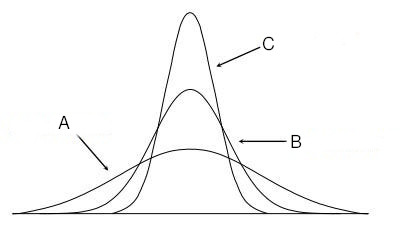
\includegraphics[width=0.4\textwidth]{../img/kurtosis.jpg}
\end{center}

\choice{A}{B}{C}{None}{a}

\question \textbf{The Range of Karl Pearson's measure of skewness --}
\choice{(0, 1)}{(-1, 1)}{(-3, 3)}{(0, $\infty$)}{c}

\question \textbf{Which can be used to measure dispersion?}
\choice{$\mu_2'$}{$\mu_1$}{$\mu_2$}{$\mu_1'$}{c}

\question \textbf{For a mesokurtik distribution, $\beta_2 = -$}
\choice{0}{-3}{3}{1}{c}

\question \textbf{Which of the following has the strongest correlation?}
\choice{-0.92}{0.67}{0.50}{0.91}{a}

\question \textbf{The lowest possible value of the correlation coefficient ---}
\choice{1}{0}{$-\infty$}{-1}{d}



\question \textbf{Which of the following is most suitable for comparing the sales of five different products over a single year?}
\choice{Histogram}{Pie Chart}{Simple Bar Diagram}{Frequency Curve}{c}

\question \textbf{Which statement is true about secondary data?}

i. Already published \\
ii. Economical \\
iii. Always up-to-date

\textbf{Which one is correct?}

\textbf{Which one is correct?}

\choice{i and ii}{i and iii}{ii and iii}{i, ii and iii}{a}
% Part 1

\question \textbf{Which of the following is an example of cyclic variation in a time series?}  
\choice{Boom and recession phases in an economy}{Increase in electricity consumption during summer}{High demand for umbrellas during the rainy season}{Sudden decline in stock prices due to a pandemic}{a}   

\question \textbf{Which measure of trend is subjective?}
\choice{Semi-average method}{Graphical method}{Moving average method}
{None of the above}{b}

\question \textbf{Which of the following is an example of an infinite population?}  
\choice{Patients in a hospital}{Water molecules in the ocean}  
{Cars on a highway}{Students in a university}{b}  

\question \textbf{How many measurement scales are there?}
\choice{2}{3}{4}{5}{c}

\question \textbf{Given $z_1=3$, $z_2=0$, $z_3=-3$, and $z_4=2$, what is the value of $\displaystyle \sum_{i=1}^4 (z_i^2 + 5)$?}  
\choice{30}{40}{35}{45}{d}  



\textbf{Answer the next THREE questions based on the following information.}

The weights of 120 fruits were recorded and this frequency distribution was constructed.

\begin{table}[H]
\centering
\begin{tabular}{c|c|c|c|c}
\begin{tabular}[c]{@{}c@{}}Weight (grams)\end{tabular} & 0-50 & 50-100 & 100-150 & 150-200 \\ \hline
No. of Fruits & 30 & 35 & 25 & 30
\end{tabular}
\end{table}

\question \textbf{How many fruits weigh at least 100 grams?}
\choice{55}{50}{60}{65}{a}

\question \textbf{How many fruits weigh less than 100 grams?}
\choice{68}{70}{65}{50}{c}

\question \textbf{What percent of fruits weigh between 50 and 150 grams?}
\choice{50\%}{55\%}{60\%}{75\%}{c}
%--------Group Ends

\question \textbf{Which measure is not used in determining skewness?}
\choice{Arithmetic Mean}{Geometric Mean}{Median}{Mode}{b}

% Multiple Completion Starts
\question \textbf{The following are values of arithmetic, geometric, and harmonic mean, respectively}

i. \{10, 12, 14\} \\
ii. \{10, 10, 10\} \\
iii. \{10, 8, 6\}

\textbf{Which one is possible?}

\choice{i and ii}{i and iii}{ii and iii}{i, ii and iii}{c}
% Multiple Completion Ends

\question \textbf{Let $Y = aX + b$, where $a$ and $b$ are constants. If $\bar X = 8$ and $\bar Y = 30$, and $a = 3$, $b = ?$.}
\choice{3}{6}{9}{12}{b}

\question \textbf{If $Q_1 = 25$ and $QD = 10$, what is the value of $Q_3?$}
\choice{45}{70}{10}{25}{a}

\question \textbf{What is the variance of a constant c?}
\choice{1}{0}{-1}{$\infty$}{b}

\question \textbf{For two values, the range is found to be 8. What are the values of mean deviation and standard deviation, respectively?}
\choice{(2,4)}{(4,4)}{(4,8)}{(8,8)}{b}


% Multiple Completion Starts
\question \textbf{Which of the following are true about variance?}

i. It is always non-negative \\
ii. It is measured in squared units of the original data \\
iii. It becomes zero when all observations are equal

\textbf{Which one is correct?}

\choice{i and ii}{i and iii}{ii and iii}{i, ii and iii}{d}
% Multiple Completion Ends

% Situation Set Starts
\textbf{Answer the next two questions based on the following information}

\begin{center}
The first and second moments of a distribution around 2 are 13 and 195, respectively.
\end{center}

\question \textbf{What is the arithmetic mean?}
\choice{15}{12}{11}{26}{a}

\question \textbf{What is its variance?}
\choice{20}{21}{26}{25}{c}
% Situation Set Ends



\end{questions}

\vspace{1cm}

\begin{center}
%“It is easy to lie with statistics; it is easier to lie without them.” \\ - Frederick %Mosteller
 \vfill 

--AAM--
\end{center}

\pagebreak
%\newpage  %Uncomment to put on new age
\bigskip

%\begin{multicols}{3}
%[
%Answer Key
%]
%\showallanswers % Phil Hirschorn
%\end{multicols}


\end{document}